\chapter{Gestion des traductions}
\section{Module de traduction}
\label{stringTranslator}
Dans certain cas, le logiciel \tria est fourni avec un module de traduction.\\

Attention, il n'est pas possible d'utiliser simultanément le module de traduction et \tria. Vous devez fermer le module de traduction pour voir le résultat dans \tria.\\

Ce module permet de traduire les chaînes de caractères qui apparaissent dans un ensemble de schémas. Ces chaînes correspondent aux noms des éléments suivants :\\

\begin{itemize}
\item Les acteurs
\item Les briques
\item Les moyens
\item Les activités
\item Les temps d'actions
\item Les étapes
\item Les objectifs
\item Les moyens\\
\end{itemize}

Le module de traduction travaille directement sur le fichier utilisé par \tria. Lorsqu'une traduction est associée à une chaîne de caractère, elle sera utilisée lors de l'utilisation suivante de \tria.

Un champ de recherche permet de filtrer les entrées affichées dans la fenêtre. La recherche est effectuée sur le terme initial et sa traduction.\\

Pour utiliser le texte initial au lieu d'une traduction, il suffit d'effacer entièrement le texte de la traduction.\\

Il possible d'importer et d'exporter une traduction depuis le module de traduction.\\

Attention, lors d'une importation, la traduction courante est perdue. Veillez à exporter cette dernière avant si vous voulez la conserver.\\

\begin{figure}[h!]
\centering
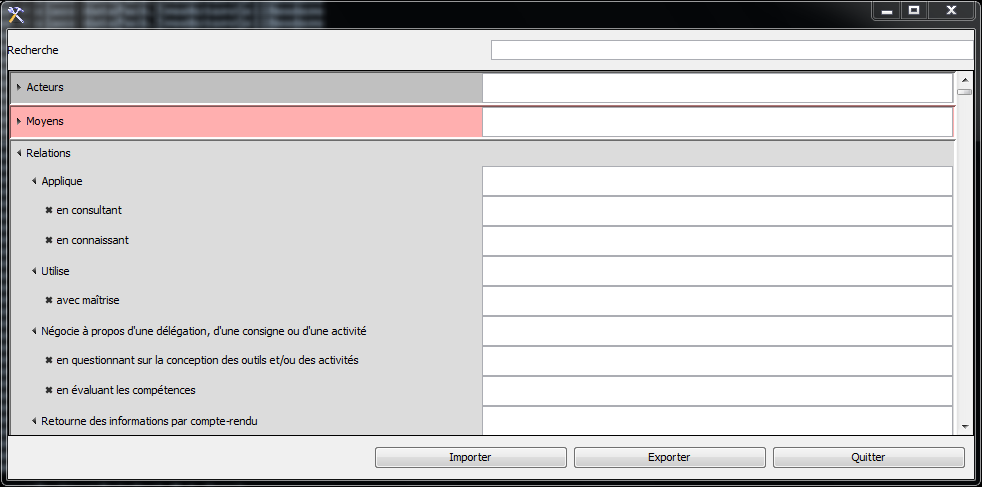
\includegraphics[width=0.5\textwidth]{images/translator.png}
\caption{L'interface du module de traduction}
\end{figure}


\section{Gestion des traductions de datapack}

Il est aussi possible de changer la traduction depuis \tria avec l'option "Changer la langue du datapack" dans le menu Edition (voir image \ref{menu_edition}). Attention, la traduction actuelle sera écrasée lors de cette opération, si vous avez commencez à réaliser un traduction, vous pouvez l'enregistrer depuis le module de traduction (voir partie \ref{stringTranlator}).\\

Il est possible d'obtenir le compte du nombre de mots et de phrases traduites à l'aide du bouton "Statistiques de la traduction" en bas à gauche de la fenêtre.\\

\section{Traduction de l'interface du logiciel}

La langue de l'interface peut être choisie à l'aide du menu "Langue" dans l'interface principale. Le logiciel doit être redémarré après un changement de langue.\\

Il est possible d'ajouter une nouvelle langue en ajoutant le fichier correspondant dans le sous dossier "language" du répertoire d'installation du logiciel. Pour réaliser cette traduction, il suffit de réaliser une copie d'un des fichier puis de traduire l'ensemble des phrases qu'il contient. La nouvelle langue sera proposée dans le menu "Langue" lors du démarrage suivant du logiciel.\\

Si des phrases sont manquantes dans un fichier de traduction, celles de la version françaises seront automatiquement utilisées à la place. De ce fait, si certaines phrases sont en français, cela signifie sûrement que leur traduction est manquante. 

